\documentclass[11pt, a4paper, twoside, openright]{article}

\usepackage{graphicx,color}
\usepackage[utf8]{inputenc}
\usepackage[justification=centering]{caption}
\usepackage{amssymb, amsmath, array, cite, float, url}

\begin{document}

% Example of title page for the projects carried out within DEDIS
% Copied from lasec 

% Simply include it in your mastex tex file: 
%        % Example of title page for the projects carried out within DEDIS
% Copied from lasec 

% Simply include it in your mastex tex file: 
%        % Example of title page for the projects carried out within DEDIS
% Copied from lasec 

% Simply include it in your mastex tex file: 
%        \input{cover}


% Updated October 2016


\newcommand{\logoepfl}[0]{
  \begin{center}
    
\includegraphics[width=4cm]{logo_epfl_coul.eps}
  \end{center}
  \vspace{0.3cm}
  \hrule
}
\newcommand{\project}[1]{
  \begin{center}
    \large{#1}
  \end{center}
  \vspace{1cm}
}
\newcommand{\department}[1]{
  \begin{center}
    \large{#1}
  \end{center}
}
\newcommand{\lab}[1]{
  \begin{center}
    \large{#1}
  \end{center}
}
\newcommand{\supervisor}[3]{
  \begin{center}
    \begin{normalsize}{
        \bf #1}\\#2\\#3
    \end{normalsize}
  \end{center}
}
\renewcommand{\author}[1]{
  \begin{center}
    \Large{#1}
  \end{center}
  \vspace{0.5cm}
}
\renewcommand{\title}[1]{
  \vspace{3cm}
  \begin{center}
    \huge{#1}
  \end{center}
  \vspace{1.7cm}
}
\renewcommand{\date}[2]{
  \begin{center}
    \normalsize{#1 #2}
  \end{center}
  \vspace{0.5cm}
}


\thispagestyle{empty}


% begin title page
  \logoepfl
  
  \title{Explore cross-platform mobile platforms}
  
  \author{Louis-Maxence Garret}
  \department{School of Computer and Communication Sciences}
  \lab{Decentralized and Distributed Systems lab}
  \project{Master Optional Project}
  
  \date{January}{2019}

  \begin{center}
    \begin{tabular}{cc}
      \begin{tabular}{p{4.0cm}}
        \supervisor{Responsible}{Prof. Bryan Ford}{EPFL / DEDIS}
      \end{tabular}&
      \begin{tabular}{p{4.0cm}}
        \supervisor{Supervisor}{Linus Gasser}{EPFL / DEDIS}
      \end{tabular}
    \end{tabular}
  \end{center}

% end title page




% Updated October 2016


\newcommand{\logoepfl}[0]{
  \begin{center}
    
\includegraphics[width=4cm]{logo_epfl_coul.eps}
  \end{center}
  \vspace{0.3cm}
  \hrule
}
\newcommand{\project}[1]{
  \begin{center}
    \large{#1}
  \end{center}
  \vspace{1cm}
}
\newcommand{\department}[1]{
  \begin{center}
    \large{#1}
  \end{center}
}
\newcommand{\lab}[1]{
  \begin{center}
    \large{#1}
  \end{center}
}
\newcommand{\supervisor}[3]{
  \begin{center}
    \begin{normalsize}{
        \bf #1}\\#2\\#3
    \end{normalsize}
  \end{center}
}
\renewcommand{\author}[1]{
  \begin{center}
    \Large{#1}
  \end{center}
  \vspace{0.5cm}
}
\renewcommand{\title}[1]{
  \vspace{3cm}
  \begin{center}
    \huge{#1}
  \end{center}
  \vspace{1.7cm}
}
\renewcommand{\date}[2]{
  \begin{center}
    \normalsize{#1 #2}
  \end{center}
  \vspace{0.5cm}
}


\thispagestyle{empty}


% begin title page
  \logoepfl
  
  \title{Explore cross-platform mobile platforms}
  
  \author{Louis-Maxence Garret}
  \department{School of Computer and Communication Sciences}
  \lab{Decentralized and Distributed Systems lab}
  \project{Master Optional Project}
  
  \date{January}{2019}

  \begin{center}
    \begin{tabular}{cc}
      \begin{tabular}{p{4.0cm}}
        \supervisor{Responsible}{Prof. Bryan Ford}{EPFL / DEDIS}
      \end{tabular}&
      \begin{tabular}{p{4.0cm}}
        \supervisor{Supervisor}{Linus Gasser}{EPFL / DEDIS}
      \end{tabular}
    \end{tabular}
  \end{center}

% end title page




% Updated October 2016


\newcommand{\logoepfl}[0]{
  \begin{center}
    
\includegraphics[width=4cm]{logo_epfl_coul.eps}
  \end{center}
  \vspace{0.3cm}
  \hrule
}
\newcommand{\project}[1]{
  \begin{center}
    \large{#1}
  \end{center}
  \vspace{1cm}
}
\newcommand{\department}[1]{
  \begin{center}
    \large{#1}
  \end{center}
}
\newcommand{\lab}[1]{
  \begin{center}
    \large{#1}
  \end{center}
}
\newcommand{\supervisor}[3]{
  \begin{center}
    \begin{normalsize}{
        \bf #1}\\#2\\#3
    \end{normalsize}
  \end{center}
}
\renewcommand{\author}[1]{
  \begin{center}
    \Large{#1}
  \end{center}
  \vspace{0.5cm}
}
\renewcommand{\title}[1]{
  \vspace{3cm}
  \begin{center}
    \huge{#1}
  \end{center}
  \vspace{1.7cm}
}
\renewcommand{\date}[2]{
  \begin{center}
    \normalsize{#1 #2}
  \end{center}
  \vspace{0.5cm}
}


\thispagestyle{empty}


% begin title page
  \logoepfl
  
  \title{Explore cross-platform mobile platforms}
  
  \author{Louis-Maxence Garret}
  \department{School of Computer and Communication Sciences}
  \lab{Decentralized and Distributed Systems lab}
  \project{Master Optional Project}
  
  \date{January}{2019}

  \begin{center}
    \begin{tabular}{cc}
      \begin{tabular}{p{4.0cm}}
        \supervisor{Responsible}{Prof. Bryan Ford}{EPFL / DEDIS}
      \end{tabular}&
      \begin{tabular}{p{4.0cm}}
        \supervisor{Supervisor}{Linus Gasser}{EPFL / DEDIS}
      \end{tabular}
    \end{tabular}
  \end{center}

% end title page


\tableofcontents
\newpage
\section{Introduction}
The purpose of this project is to implement and improve blockchains storage and transactions of accounts, and witness validation of those operations. More precisely, this project has two objectives. The first objective is to add a documented transaction batching library to Omniledger\cite{Omniledger}. The second objective is to improve ByzcoinX\cite{Byzcoin}, by reducing the running time in the most frequent situations by a large factor. Omniledger will be presented in section~\ref{Omniledger} and ByzcoinX in section~\ref{ByzcoinX}.

This project's main purposes are the following:
\begin{itemize}
\itemsep0em
\item Have clear and reusable code for current and future projects. 
\item Make ByzcoinX more efficient for encouraging its use.
\end{itemize}

The next section will present Omniledger, the blockchain for which all of those technologies are implemented and Merkle trees, a data structure that is the basis upon which transactions are done.

%It follows the two main project areas: the collection, a Merkle tree key-value pair data-structure and the CoSi protocol and its quick answer optimisation.
\subsection{Omniledger}
\label{Omniledger}
Omniledger\cite{Omniledger} is a blockchain developed by the Decentralized and Distributed Systems laboratory of EPFL. It is a Distributed Ledger that insures decentralisation, security and scalability. Every block of Omniledger is defined mainly by a state which is stored on a collection, a Merkle tree like data-structure explained in section \ref{merkle_tree}. This collection contains the balance of every account on the blockchain at a given block's time. The first part of the project consists in the improvement and cleaning of the collection's code.Omniledger also appoints a leader node (which may change), to which updates of the blockchain state will be proposed. When such a proposition arise, the leader asks other nodes to validate or reject the update. To be able to do this verification in a scalable and robust way, the ByzcoinX protocol is used. Both those systems, the collection and the ByzcoinX protocol will be described in details in the next section.

\subsection{Merkle trees}
\label{merkle_tree}
Omniledger stores key-values pairs using a data structure called Merkle \mbox{tree\cite{Merkle_tree}}. A Merkle tree, also called hash tree, is a tree data-structure as shown on figure \ref{fig:Merkle_tree}.
\begin{figure}
 \centering
  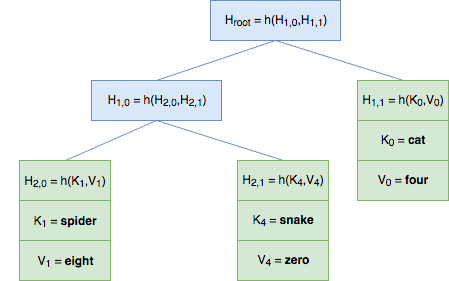
\includegraphics[width=9cm]{merkle_tree.png}
  \caption{Example of a Merkle tree}
  \label{fig:Merkle_tree}
\end{figure}
Every node in the Merkle tree is defined by four main elements:
\begin{itemize}
\itemsep0em
\item A label, the main feature of a Merkle tree
\item A key-value pair (in Omniledger only in the leafs)
\item Pointers to its children
\item A pointer to its parent
\end{itemize}
As shown in figure \ref{fig:Merkle_tree}, each node of the tree is labelled by a hash of the concatenation of its child nodes label and its data. The overall tree can therefore be defined mainly by its root node (containing pointers to other nodes) and the type of values it stores. Note that the Merkle tree implementation of Omniledger stores the key-value pairs only on the leafs of the tree, and not on the intermediary nodes.

\section{Architecture}
This section presents the architecture of the project. That is the practical basis upon which the project was built.

Since a major part of the project was to understand in depth the structure of the collections, this will be reflected here by going more in depth into its inner working. Therefore, the first part will present the collections in details. The second part will present the ByzcoinX protocol, which was improved as part of this project.
\subsection{Collections}
Omniledger uses collections to store the state of different accounts at a given time. Each account id is used as a key and stores in its associated value, a contract id and some data used by the contract.

\subsubsection{Merkle Patricia Trie}

The account information are not stored randomly on the Merkle tree, indeed we use the equivalent of a Merkle Patricia Trie\cite{trie}. As a hash is a suit of zeroes and ones, we start from the root and interpret a zero as ``take the left branch" and a one as ``take the right branch". This process uniquely defines the position of a key-value pair by the hash of its key. \label{key_location} The presence of any key-value pair in the tree can easily be proved by successive hashing, following the hash of the key. The first leaf encountered will either be the key we want to prove the presence or another key if the searched key is absent.

\subsubsection{Non-modifying operations}
Multiple operations can be defined on the collection. Some operations let the collection in the same state as before the operation, like searching for a key or generating a proof of inclusion. There is also modifying operations, which will be described in the next section.

One of the most common operation on a collection is to search for the value associated with a given key. Since every node location is uniquely defined by the hash of its key as described in section \ref{key_location}, there is only one path we can follow to get to a location. When a search is requested, a \textit{navigator} object is generated. This object will navigate the collection until it finds a leaf. It will then return a \textit{record} object.

\textit{Record}s are objects containing the result of a search query. They can be queried to get wether the record matches the query that generated it or if record does not match the query (when the searched key was absent from the collection). They can also obviously return the key, values that the \textit{record} contains.

One heavy operation on the collection is to prove the presence or absence of a given key in the collection. To do that, a method of the collection allows to generate a \textit{getter} object. This getter can generate two other objects: a \textit{record}, as explained previously, or a \textit{proof}.

The \textit{proof} object is more complicated. It contains the proof of inclusion of every node of the Merkle tree in the path from the root to the given key. That is a list of every hash that has to be done to go to the key's location on the tree. Each of these step is comprised of everything needed to verify the hash of the node, that is a left and right child hash and the data of the node. Since every key's location on a collection is unique, the final step of the \textit{proof} can easily prove if the location contains or doesn't contain the given key. This proves the presence or absence of a given key in the collection.

Using a \textit{proof} object, any key presence or absence can be proved by anyone, in or outside Omniledger. The \textit{proof} can also be entirely verified step by step by a \textit{verifier}. The \textit{verifier} will redo the hash of every step of the \textit{proof} to verify that they all generate the correct result.

\subsubsection{Transactions}
\label{transactions}
The collection is also able to perform modifying operations called \textit{transactions}. The state before and after the transaction must be valid, including keeping ordered key hashes. Since transactions can modify multiple nodes and are non-atomic, they are always done with a backup. This backup allows an easy rollback if any phase of the transaction fails. The transaction always ends with a verification and fixing of the collection. That way we are certain that a transaction will never break the collection.

There is currently four types of transactions implemented:
\begin{itemize}
\itemsep0em
\item Adding a new key-value pair
\item Updating the value associated with a given key
\item Updating only one of the multiples values that can be associated with a key
\item Removing a key-value pair
\end{itemize}

Each of those \textit{transaction}s, if successful, will modify the hash of the root of the collection and every node in the path to the node modified by the transaction.

All \textit{transaction}s also require to first prove the presence or absence of a key in the collection in order to perform an operation on it. That is why we cannot perform \textit{transaction}s naively in parallel. To allow multiple computers to propose \textit{transaction}s concurently, we need to be able to handle multiples \textit{transaction}s that each starts with the same state (latest block). That is the purpose of \textit{update} objects. An \textit{update} contains a list of \textit{transactions}. When applied, an \textit{update} first perform the proof needed for every \textit{transaction}. Then it removes invalid \textit{transaction}s, for example adding and already present node or setting a new value to an absent node. And finally, it applies all \textit{transaction}s sequentially. \textit{Transaction}s are first-come, first serve. Meaning that in some cases there will be incoherent \textit{transaction}s. For example, a removal, followed by a modification of the removed node can occur. In that case, the second \textit{transaction} is ignored. In the future, more clever ways could be used to determine transactions order, see section \ref{future_works}.

\subsection{CoSi}
CoSi\cite{CoSi} is a signature protocol allowing a computer to sign a given proposal using other independent witnesses. In Omniledger the proposal to be signed is a collection update. This protocol makes proposal signing not dependent on a single entity, the computer signing the proposal, but instead certify that a certain number of witnesses have validated the proposal. The protocol is scalable by using two main optimisation. First a communication tree between the witnesses. This communication tree allows a distribution of the connexions on lots of nodes and not only the root. Indeed, a root connecting individually with every witness will soon meet its bandwidth limit and not scale linearly relative to the number of witnesses. The second optimisation is the use of Schnorr Signatures\cite{Schnorr}, which is a method to aggregate signatures to have a final signature size fixed and independent of the number of witnesses. The protocol takes as input mainly an Omniledger update to be signed and outputs an easily verifiable aggregate signature validating it. The signature is only computed if two third of the nodes accepts the proposed update. The protocol can also output a rejection if the two-third threshold can not be reached because of too many refusals. To verify this signature aggregate, one only needs to know every witnesses' public keys.

More specifically, the protocol uses four messages in two round-trip, starting at the root.
\begin{enumerate} 
\itemsep0em
 \item \textbf{Announcement:} The leader announce the start of the protocol and sends the proposal down the tree.
\item \textbf{Commitment:} Each node accepting the proposal generates a Schnorr commitment and its corresponding secret. It then aggregate its commitment with their children's commitment (if any) and sends the aggregate to its parent.
\item \textbf{Challenge:} Once the root received enough commitments, it generates a Schnorr challenge and send it down the tree.
\item \textbf{Response:} In this last phase, every committed node generates a response, based on the collective challenge, its commitment, its secret number and its private key. It then aggregates this response with its children responses (if any) and sends it up the tree, as the commitment in phase 2.
\end{enumerate}
Lastly, the aggregated responses and the aggregated commitments are used to sign the proposal.

This protocol therefore returns a global signature, insuring that a certain number of nodes have validated a proposal.

\subsubsection{ByzcoinX}
\label{ByzcoinX}
In Omniledger, we use a variation of the CoSi algorithm, called ByzcoinX, that uses a three layer tree. The first layer is the root, the second layer is the \textit{subleader}s and the third layer is the leafs. This three level tree allows a nice balance between two factors. If the tree has too many layers, the time it takes for a round-trip down and up the tree will be a performance bottleneck. If, on the other hand, all nodes are connected to the leader (a two level tree), then the leader's performance will be the bottleneck. Thus, ByzcoinX uses a three layer tree.

\section{Implementation}
\subsection{Collection Code cleaning}
The first task, once the collection structure was understood and its inner workings known, was to comment its whole public interface. Every public method, function and structure was documented to allow an easier use in the future.

Then the code was cleaned by making it compliant to Go Lint\cite{Golint}, Go fmt\cite{gofmt} and using a standardised naming convention. Those operations are detailed in the next paragraph.

Golint is a linter for the Go language that flags potential errors of coding style. It is used by most of DEDIS projects. Golint flagged numerous coding style errors in the code. The most common ones were putting \textit{else} keyword after a terminating \textit{if} condition, use of reserved keywords and incorrect formatting of error messages. Go fmt automatically formatted the code to use the canonical Go style. Finally, names were modified to use camel case and some variables names were simplified. All those changes insured a greater readability of the code therefore facilitating review and work of other persons on the code.

\subsubsection{Hashing}
The collection library, before the project, was using its own implementation of concatenation and hashing, using around 400 lines of code. The decision was made to use known libraries instead. Most precisely Protobuf \cite{protobuf} and sha256 libraries. This decision was made because:
\begin{itemize}
\itemsep0em
\item It allows an easier translation of the code to another programming language, which is planned for Omniledger.
\item It decreases bugs probability by using public and tested libraries.
\item It avoids code duplication
\end{itemize}
To generate the hash of a node, the node elements to be hashed are put in a structure. This structure is then encoded into an array of bytes using Protobuf. Finally, this array of byte is hashed to generate the node label. All this is done using 15 lines of codes instead of 400, thanks to the libraries use.

\subsubsection{Bug corrections in collections}
The reading of the whole collection code allowed multiple bugs to be unveiled. For example, some errors were discarded instead of being correctly forwarded. This prevented the good understanding of multiples common errors. Another unveiled bug was the adding of empty keys to the collection which was not prevented. This adding put the collection in an unstable case as a failing search generated a \textit{record} with a nil key. This \textit{record} described the nil key as present in the collection. Therefore, every search in a collection which contained an empty key returned the search query as successful. Both those bugs were corrected.

\subsection{ByzcoinX Quick answers}
One of the major time constraints for ByzcoinX is waiting for the answers of the announcement (such answers are called ``commitment") as shown on figure~\ref{fig:CoSi}. The basic ByzcoinX algorithm will only end the commitment phase when every leaf have answered or when they timeout. This behaviour allows to have the maximum number of signatories in a given time period. However, the time to get an answer is equal either to the timeout or to the answer time of the slowest node. Since, in the basic use case, with thousands of witnesses, it is very probable for at least one node to be offline, the protocol time will often be at its slowest, that is waiting on the timeout.
\begin{figure}
 \centering
  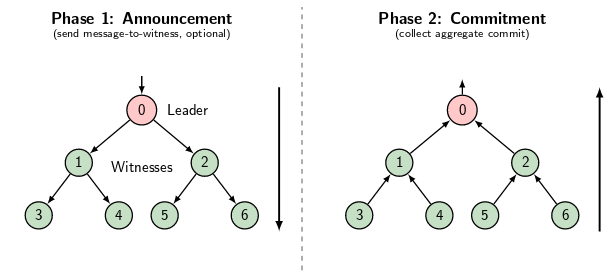
\includegraphics[width=\textwidth]{CoSi_Announcement_Commitment.png}
  \caption{First two phases of the CoSi protocol}
  \label{fig:CoSi}
\end{figure}

To speed-up the process, we give the threshold at the start of the protocol. The root then divides the threshold by the number of subleaders. The subleader threshold is added in the initial message (the announcement). As soon as a subleader gets enough commitments from its children to reach the threshold, it sends the aggregated commitments to the root, not waiting for every commitments. The subleader also sends a final commitment once every child has answered or the timeout has elapsed.

The root receives commitments normally from every subleader. If it gets a second commitment from a node that already sent a quick commitment, it replaces the quick commitment by the new, bigger one. As soon as the root reaches the threshold, it passes to the next phase, without waiting for the commitment of every node.

Note that sometimes, the threshold cannot be reached. This is the case mostly when nodes refuses an invalid update proposal. When a subleader detects that its threshold cannot be reached, it sends back a quick answer as well. This answer will contain the number of refusal. It will, as in the normal case, also sends back a final answer, once every node has answered or the timeout is reached. The root will, as for the commitments, count the total number of refusals. If the threshold cannot be reached, the root will abort the process and send back to the caller a signature refusal.

This optimisation makes the ByzcoinX average commitment time go from almost always the timeout to the time it takes the two-third quickest node to answer. This is a huge improvement.


\subsection{Simplified code workflow}
The subleader code had to be completely changed to implement the quick answer optimisation. Indeed, in the unoptimised ByzcoinX , the subleader was waiting for either commitments from every one of its children or a timeout. When everything was received or the timeout reached, the subleader added its own commitment to the commitment list, aggregated them and send the aggregate to its parent. The subleader then waited on the challenge. This process was a very ``waterfall" model, with defined order.

However, with the ByzcoinX optimisation, the subleader is not guaranteed which even will come first. It can receive the challenge, commitments or the timeout signal in different order. Once the quick answer has been sent, the subleader should continue to gather commitments and wait on the timeout, while at the same time be ready to receive a challenge if the root succeeds at reaching the threshold.

Therefore, the subleader waits on the three channels at the same time: the commitments from the children, the challenge from the root and the timeout signal. To simplify even further, the subleader's own commitment is generated in parallel, after the node has validated the update proposal. This parallel commitment is then sent on the same channel as other commitments, being treated as any other commitment and avoiding code duplication. Every time the subleader receives a new commitment or refusal, it checks if the threshold is reached and sends the aggregated commitment if that is the case or if the threshold is not reachable anymore. It then continues to receive commitments until the challenge is received from the root. It then goes to the last phase normally.

All this unified process simplifies a lot the code by preventing multiple code repetition and handling all commitments the same way.

\subsection{Additional defences against malicious nodes}
During the update of the ByzcoinX code, multiple potential vectors of attacks have been corrected to insure a greater security.

The main added protection concerned the commitment masks. When a node generates its commitment or an aggregated commitment, it also generates a mask, basically, a list of zeroes and ones that indicate which nodes are in the aggregated commitment. A verification of leafs mask was added instead of blindly merging the received masks. That way, we prevent rogue nodes from failing the whole signature process.

The second added protection is insuring that the ByzcoinX protocol is now launched on a maximum three level tree. Indeed, if the protocol is launched on a more than three level tree, then the code will fail in multiple places. For example, the personalised threshold for each branch will be invalid, or the mask verification will fail. The simple added tree depth assumption allows a far simpler code overall by removing the need of generalisations and countless edge cases.

Finally, multiple additional checks are done all along the ByzcoinX process to insure that a faulty state does not propagate further. For example, the number of commitment and refusals received is checked to insure that it is always below the number of witnesses a nodes is responsible for. Another example is the threshold that is checked in every step to insure a correct quick answer behaviour, and adversary node or interception protection.

\subsection{Unit tests and documentation}
Since the purpose of the whole project was to have a code base that is easily reusable, the whole project was made with a strong emphasis on documentation, unit testing and code readability. Therefore, every public method was documented with the latest changes and unit tests were updated.

We should note that even though unit testing can be quite extensive, unit tests can always be added. Moreover, having lots of unit tests does not guarantee a bug-free code as real-life conditions can be quite different than planned scenarios. Nevertheless, Unit tests allowed a big reduction in the number of bugs in the code.

\section{Results analysis}

To analyse the performance gained by using the quick answer paradigm for ByzcoinX, a performance test was created. The simulation was launched with a basis of 50 nodes and 6 subtrees (6 subleaders), using the Omniledger default leafs timeout of 417ms. We intentionally keep the number of machines to 50 to avoid any overhead by the testbed limitation. The threshold used is the default Omniledger threshold of two thirds, which implies a threshold of $ {\lceil 50 \cdot 2/3\rceil} = 34$ nodes. To get a better approximation, the result is the average of 10 tests. The network delay are of 0ms. Adding a network delay will add a constant time to every value as the number of network link is always the same. 

We then vary the number of failing nodes between $0, 1, 2, 5, 10, 11 \text{ and } 16$ (16 being the maximum allowing us to reach the threshold). The running time is measured from the start signal of ByzcoinX to the final signature sending.
\begin{figure}
 \centering
  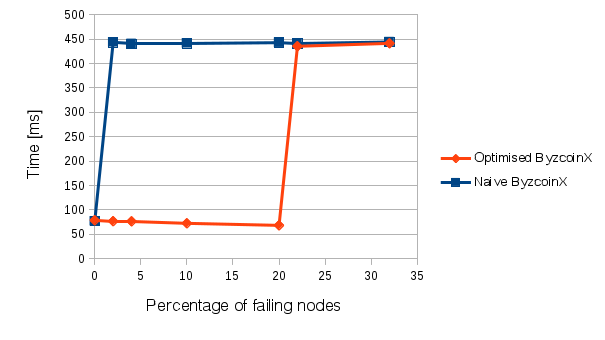
\includegraphics[width=\textwidth]{time_ByzcoinX.png}
  \caption{Comparison of naive and optimised ByzcoinX running time in function of the number of failing nodes}
  \label{fig:performance}
\end{figure}

We can see in Figure~\ref{fig:performance}, that in the naive ByzcoinX, as soon as one node is failing, the whole process is capped by the leafs timeout. Then, no matter how many failing nodes there is, the time is always similar, that is limited by the timeout. This is consistent with the result obtained in the CoSi implementation paper\cite{CoSi_implementation}.

The optimised ByzcoinX has approximately the same running time as the naive version when every node is succeeding. However, if one node fails, the performances are not impacted. Indeed, the threshold is reached before getting a timeout from the failing node. This short running time is present until approximately $20\%$ of nodes are failing. At that point, the quick answers are barely not able to reach the threshold anymore. Therefore the algorithm waits for the timeout.

The switching point between short running time and long running time for the optimised version is not exactly at the threshold. That is because the failing nodes are not spread evenly among branches. Therefore, we will almost never be in the optimal case where every subleader just reaches the threshold. That is why the switching point will in practice always be a little less than the threshold.

\section{Future work}
\label{future_works}
A lot can still be added to improve the project.
\begin{enumerate}
\item Add backward compatibility with the naive ByzcoinX. That way, we can still require a signature from ByzcoinX even if the threshold is not reached.
\item Store the collections on the hard drive instead of just the memory. That way, if the program closes, we don't have to fetch the collections again from the blockchain.
\item Rework the ByzcoinX timeouts to make them more consistent. A great job has been done on this previously, but more thinking is still necessary to have an optimal system.
\item Improve the ByzcoinX protocol, for example by allowing a root node failure or by better detection and removal of adversarial nodes.
\item Handle conflicting lists of \textit{transaction}s more finely. Currently, a conflicting one is blindly removed, which is not ideal.
\item Add more unit tests and improve the unit test coverage. This can always be done and insures a more stable code.
\end{enumerate}

\section{Installation}
The ByzcoinX code is publicly available at \url{https://github.com/dedis/cothority}. The ONet and Kyber libraries are also required. To get everything, the easiest way is to do a \textit{go get} \textit{https://github.com/dedis/cothority}\\ \textit{https://github.com/dedis/onet} \textit{https://github.com/dedis/kyber}

The main ByzcoinX protocol code is in the folder ``ftcosi/protocol". There, there is two main protocols, the root node protocol (\textit{protocol.go} and \textit{protocol\_commitments.go}) and the other nodes subprotocol (\textit{sub\_protocol.go}).
 
To run a ByzcoinX simulation, simply follow the \textit{README} instructions. You can modify the parameters of the simulation in the \textit{local.toml} file.

The collections are currently implemented on the folder ``omniledger/ collection" on \url{https://github.com/dedis/student_18_omniledger} but will soon be merged onto a final DEDIS repository. A \textit{README} also explains how to use the collections.

\section{Conclusion}
The purpose of this project was to implement reusable collections and quick witness cosigning, to use mainly in Omniledger. This has proven quite a success. The collections are now fully commented and even improved. The ByzcoinX witness cosigning protocol was also quite improved and is now much more efficient, as shown by the performance tests. 

This project has produced a clean and efficient code that will be used in multiple softwares in the future.

\subsection{Personal experience}
Even though there is always more than can be done, I am overall satisfied by this project. Indeed, I had to dive into a code base that I was unfamiliar with and work to be efficient and give reusable results. I have learned a lot through this project and all those skills will prove precious for the future. I am proud of the results of this project.

\section{Bibliography}
\bibliographystyle{unsrt}
\bibliography{biblio}
\end{document}
